\chapter{\label{chap:Introduction}Introduction: Effective Theories}

The concept of an effective theory is ubiquitous in physics when a problem involves multiple scales. Fundamentally, the idea is to solve an intractable problem by forming an expansion in the ratio of these scales, then neglecting all but a finite number of terms. This of course requires that the ratio be small, or that the scales are well separated. The truncated expansion should simplify the solution while still retaining predictive power at the scales of interest. We can think of Newtonian mechanics as such an approximation to the theory of special relativity, expanded in the ratio of relevant velocities to the speed of light. Introductory electrodynamics courses often start by considering point charges, essentially the first term in a multipole expansion of the size of the charge distribution compared to the distance from said distribution.

Although these simplifying approximations have a long history in physics,  the work of Wilson \cite{Wilson197475} in the 1970s paved the way for a more rigorous modern perspective in quantum theories. From a contemporary viewpoint, effective field theories are useful either when the details of physics above some energy scale $\Lambda$ (or below some length scale) are unknown or when the observables of interest are insensitive to such physics. For example, it is believed that the standard model of particle physics is an effective theory. Infinities, which are removed by renormalization, arise because there is some energy scale at which new physics comes into play and the model is therefore not to be taken seriously at arbitrarily high energies when unknown physics contributes significantly. Furthermore, not all of the standard model particles and interactions are relevant for all physical phenomena. We can therefore formally generate new effective theories systematically from the standard model by integrating out degrees of freedom such as very massive particles. 

Fermi's original theory of beta decay is an excellent example of how this works in practice. In Fermi's time, the $W$ gauge bosons of the electroweak interaction (with masses around 80 GeV) were unknown. At the same time, experiments were probing the nuclear beta decay only at very low energies on the order of tens of MeV. In ignorance, Fermi proposed a pointlike four Fermion interaction to describe the reaction which was very successful because the separation of the experimental energy scale and the electroweak scale was so large. Of course, we now know the details of the electroweak theory and can perform calculations accurately at or above the $W$ boson mass\footnote{Note that evaluating beta decay observables from a theory exactly consistent with QCD excitations is an unsolved problem.}. On the other hand, such calculations are significantly more difficult than the original Fermi theory which can be now be recovered in a principled way by integrating out the vector bosons. When calculating beta decay lifetimes at energies far below the electroweak scale, it would be wise to prefer the simpler effective theory which is, in any case, still incredibly accurate. 

Weinberg pioneered another approach to generating an effective field theory describing interactions of hadrons \cite{WEINBERG1990288} from the bottom up rather than by integrating out degrees of freedom. In his framework, one should consider all possible terms which respect the approximate chiral symmetry of quantum chromodynamics (QCD) at low energies. Since there are an infinite number of such terms, a power counting scheme is necessary to group interactions into a finite numbers of terms at each order in a low-momentum expansion\footnote{The relevant expansion parameter is $Q/\Lambda_{\text{QCD}}$ where $Q$ represents some small momentum scale and the chiral symmetry breaking scale $\Lambda_{\text{QCD}}\approx 1\text{GeV}$.}. The expansion contains a number of parameters, called low energy constants (LECs), multiplying the various terms. These are constrained by the chiral symmetry, and their values are determined by fitting calculated observables to their experimental values. When performing calculations, one should also take the energy cutoff $\Lambda_{\text{QCD}}$ seriously as an ultraviolet cutoff (we have no reason to extend our model beyond this scale) \cite{Epelbaum2013}. 

Weinberg's approach, referred to as chiral perturbation theory (ChPT), has enjoyed significant popularity in the nuclear physics community. Derivation of a non-relativistic potential describing the interactions of nucleons is a primary goal of the field, and the separation of scales which makes effective theories useful had long been observed in attempts at generating such a potential phenomenologically (see \Cref{fig:NuclearPotential}). The accuracy of chiral potentials combined with their rigorous basis on underlying symmetries helped them to largely supplant the phenomenological potentials previously in use. For a thorough introduction to the subject, see \cite{Machleidt20111}.

\begin{figure}
\centering
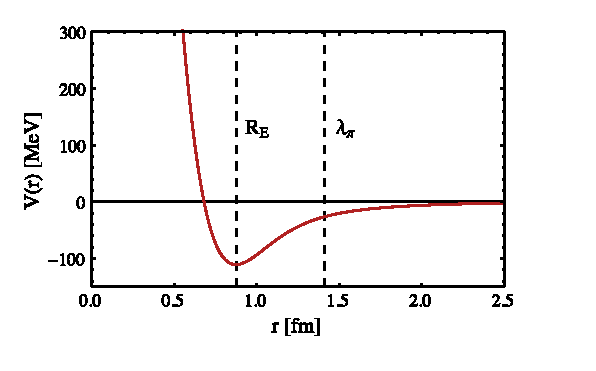
\includegraphics[scale=1.0]{Introduction/Figures/OneSZero}
\caption[Separation of scales in the two-nucleon potential]{\label{fig:NuclearPotential} The phenomenological Argonne v18 $n$-$n$ potential in the $^1S_0$ channel \cite{PhysRevC.51.38}. Note the hard core of the potential, which is strongly repulsive starting around the nucleon charge radius $R_E$, and the soft long-range attraction beyond the pion's Compton wavelength $\lambda_\pi$. Between these scales, the potential is dominated by the exchange of multiple pions and heavy mesons such as the $\rho$.  } 
\end{figure}

One generic feature of effective theories is the generation of interactions between three or more particles, even when the underlying potential is purely two-body \cite{RevModPhys.85.197}. For a long time it has been seen that the two-body terms in the nuclear potential are relatively more important than three-body interactions, which are in turn stronger than the four-body terms and so on. One great advantage of the ChPT is that it puts this observation on solid theoretical ground. The power counting shows that the three-nucleon force (3NF) first appears\footnote{Actually, the naive power counting suggests that three-body diagrams appear at NLO, but these are known to be shifted to higher orders by approximate cancellation with two-nucleon diagrams\cite{PhysRevC.49.2932}.} at $\mathcal{O}(Q/\Lambda_{QCD})^3$, known as next-to-next-to-leading order (N$^2$LO). Likewise the 4NF appears first at N$^3$LO, establishing a hierarchy of the N-body forces in nuclear physics. The first several orders of the ChPT diagrams are shown in \Cref{fig:chiralPotentialDiagrams}.

\begin{sidewaystable}\centering
\renewcommand{\arraystretch}{2.5}
\begin{tabular}{ c | c | c | c }
& 2NF & 3NF & 4NF\\ 
%%%%%%%%%%%%%%%%%%%%%%%%%%%%%%%%%%
\hline 
\begin{minipage}[c][2cm][c]{2cm}\centering LO \\ \vspace{.3cm}$\mathcal{O}\left(\frac{Q}{\Lambda}\right)^0$   \end{minipage} &  \parbox[c][][c]{5.8cm}{\centering
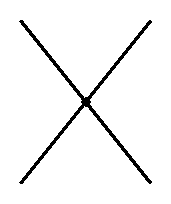
\includegraphics[scale=0.55,page=1]{Introduction/Figures/LO} 
\includegraphics[scale=0.55,page=2]{Introduction/Figures/LO}
} & &  \\
%%%%%%%%%%%%%%%%%%%%%%%%%%%%%%%%%%
\hline
\begin{minipage}[c][2cm][c]{2cm}\centering NLO \\ \vspace{.3cm}$\mathcal{O}\left(\frac{Q}{\Lambda}\right)^2$   \end{minipage} &  \parbox[c][][c]{5.8cm}{\centering
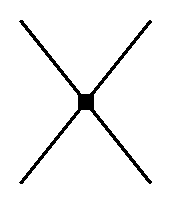
\includegraphics[scale=0.55,page=1]{Introduction/Figures/NLO}
\includegraphics[scale=0.55,page=2]{Introduction/Figures/NLO}
\includegraphics[scale=0.55,page=3]{Introduction/Figures/NLO}
\includegraphics[scale=0.55,page=4]{Introduction/Figures/NLO}
\includegraphics[scale=0.55,page=5]{Introduction/Figures/NLO}
} & &  \\
%%%%%%%%%%%%%%%%%%%%%%%%%%%%%%%%%%
\hline
\begin{minipage}[c][2cm][c]{2cm}\centering N$^2$LO \\ \vspace{.3cm}$\mathcal{O}\left(\frac{Q}{\Lambda}\right)^3$   \end{minipage} &  \parbox[c][][c]{5.8cm}{\centering
\includegraphics[scale=0.55,page=2]{Introduction/Figures/N2LO}
\includegraphics[scale=0.55,page=3]{Introduction/Figures/N2LO} 
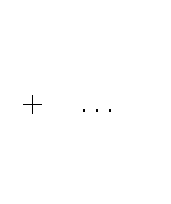
\includegraphics[scale=0.55,page=1]{Introduction/Figures/ellipsis} 
%$+\dots$
}  &  
\parbox[c][][c]{5.8cm}{\centering
\includegraphics[scale=0.55,page=4]{ChiralPotential/Figures/3NFDiagrams}
\includegraphics[scale=0.55,page=3]{ChiralPotential/Figures/3NFDiagrams}
\includegraphics[scale=0.55,page=2]{ChiralPotential/Figures/3NFDiagrams}
} & \\
%%%%%%%%%%%%%%%%%%%%%%%%%%%%%%%%%%
\hline
\begin{minipage}[c][2cm][c]{2cm}\centering N$^3$LO \\ \vspace{.3cm}$\mathcal{O}\left(\frac{Q}{\Lambda}\right)^4$   \end{minipage} &  \parbox[c][][c]{5.8cm}{\centering
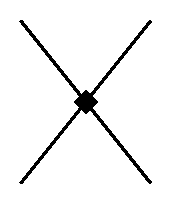
\includegraphics[scale=0.55,page=1]{Introduction/Figures/N3LO}
\includegraphics[scale=0.55,page=2]{Introduction/Figures/N3LO}
\includegraphics[scale=0.55,page=3]{Introduction/Figures/N3LO}
\includegraphics[scale=0.55,page=4]{Introduction/Figures/N3LO}
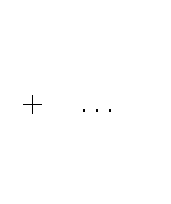
\includegraphics[scale=0.55,page=1]{Introduction/Figures/ellipsis} 
%$+\dots$
}  &  
\parbox[c][][c]{5.8cm}{\centering
\includegraphics[scale=0.55,page=5]{Introduction/Figures/N3LO}
\includegraphics[scale=0.55,page=6]{Introduction/Figures/N3LO}
\includegraphics[scale=0.55,page=7]{Introduction/Figures/N3LO}
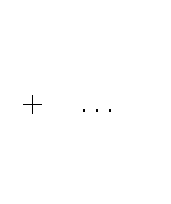
\includegraphics[scale=0.55,page=1]{Introduction/Figures/ellipsis} 
%$+\dots$
} &
\parbox[c][][c]{5.8cm}{\centering
\includegraphics[scale=0.55,page=8]{Introduction/Figures/N3LO}\hspace{.2cm}
\includegraphics[scale=0.55,page=9]{Introduction/Figures/N3LO}\hspace{.2cm}
\includegraphics[scale=0.55,page=10]{Introduction/Figures/N3LO}
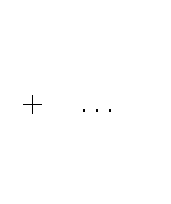
\includegraphics[scale=0.55,page=1]{Introduction/Figures/ellipsis} 
%$+\dots$
} \\
\end{tabular}
\caption[Selected Feynman diagrams for the chiral potential to N$^3$LO.]{\label{fig:chiralPotentialDiagrams} Selected Feynman diagrams for the chiral potential to N$^3$LO. Note especially the hierarchy of forces as the 3NF and 4NF first enter at N$^2$LO and N$^3$LO, respectively. Small dots, large dots, squares, and diamonds indicate vertex indices of $\Delta_i = 0,1,2,3$ respectively. The vertex index is defined as $\Delta_i=d+\tfrac{n}{2}-2$, where $d$ is the number of derivatives or pion mass insertions and $n$ the number of nucleon field operators.}
\end{sidewaystable}

Although they are not the leading terms in the expansion, the 3NF is known to be crucial to explaining observed binding energies of light nuclei \cite{ABNCSM,PhysRevC.87.014327, PhysRevLett.99.042501,0954-3899-39-8-085111} and nuclear matter \cite{Krewald2012322,PhysRevC.82.014314}. Inclusion of few-body forces beyond the 2NF is, however, quite computationally demanding. As an approximation, Chapter \ref{chap:3to2} describes a procedure for generating two-body density-dependent potentials which approximate the three-body interactions of the chiral potential at N$^2$LO. Unfortunately, this procedure generates non-locality in the coordinate space potentials which again increases the complexity of the computational problem. In Chapter~\ref{chap:localExpansion} we describe initial efforts towards a possible solution of this problem by performing an expansion of the density-dependent potentials in purely local operators.

Effective theories are also useful in completely non-relativistic formulations of quantum physics, although this is often less appreciated than for their applications in field theories. The primary features of an effective theory which we want to preserve from the rigorous field-theoretic perspective are \cite{Lepage:1997}:
\begin{itemize}
\item Include the correct low energy (long-range) physics explicitly. 
\item Identify a cutoff energy for the theory. This should lie between the low energy physics, which are known, and the unknown or intractable high energy physics. 
\item Incorporate the unknown high energy (short-range) physics by adding additional, model-independent terms and fitting the cutoff-dependent coefficients to physical observables.
\end{itemize}

From one viewpoint, a hard momentum cutoff is equivalent to reducing the basis states in momentum space used in calculations. We can thus equivalently think of restricting our calculations to a finite subspace in the full Hilbert space. This point of view is often taken for practical reasons in numerical calculations. The only other basis in which center of mass and relative coordinates cleanly separate for the N-body problem is that of harmonic oscillator (HO) eigenstates, and naturally we can also consider imposing the energy cutoff by including only HO shells with energy less than $\Lambda$. 

A detailed description of harmonic-oscillator-based effective theory (HOBET) is given in \cite{PhysRevC.77.034005}. A particular issue with using a finite basis of Harmonic oscillator states to regularize is that the states do not accurately represent very low momentum states (it is an expansion around $k\sim 1/b$). Additional corrections are therefore needed to properly treat the long-range part of the potential exactly, and these introduce an energy dependence to the effective Hamiltonian in the finite basis.

In Chapter \ref{chap:SOC}, we consider a special case of the harmonic-oscillator-based effective theory. For cold atom systems, the confining potential is often approximately harmonic. The machinery of the HOBET greatly simplifies in a harmonic confining potential, as there is no need to perform the long-range corrections. We therefore use the effective theory to non-perturbatively explore the two-body spectra of spin-$1/2$ fermions in isotropic harmonic traps with external spin-orbit potentials. Interatomic potentials are very short-ranged compared to the wavelengths of the atomic gasses at these very low temperatores, and are absorbed into short range two-body interactions fit to the two-body scattering length. Results are presented for experimentally realistic forms of the spin-orbit coupling: a pure Rashba coupling, Rashba and Dresselhaus couplings in equal parts, and a Weyl-type coupling. The technique is easily adapted to bosonic systems and other forms of spin-orbit coupling.